\documentclass{beamer}
\usepackage[utf8]{inputenc}
\usepackage[slovene]{babel} %in this stupid version of latex this is unreckognized ... :S
\usepackage[T1]{fontenc}

\usepackage{amsmath, amssymb, graphicx, float, latexsym}

%optional packages
%\usepackage{slashed, stackrel, subcaption, pdflscape}

\usetheme{Warsaw}
\logo{
	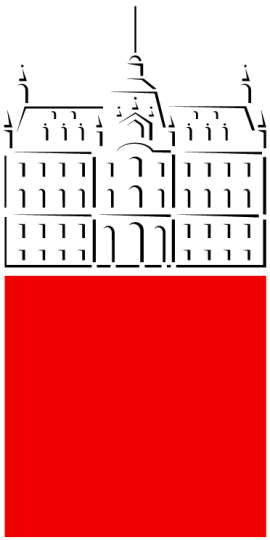
\includegraphics[keepaspectratio=1, width=0.08\textwidth]{Pics/uni-lj.png}
}

\newcommand{\F}{
	\ensuremath{\vec{F}}
}

\newcommand{\E}{
	\ensuremath{\vec{E}}
}

\newcommand{\B}{
	\ensuremath{\vec{B}}
}

\newcommand{\w}{
	\ensuremath{\omega}
}

\renewcommand{\div}{
	\ensuremath{\vec{\nabla}\cdot}
}

\newcommand{\rot}{
	\ensuremath{\vec{\nabla}\times}
}

\newcommand{\grad}{
	\ensuremath{\vec{\nabla}\times}
}

\title{Masivna elektrodinamika}
\author{Jože Zobec}
\date{Ljubljana, \today}
\institute{Mentor: Borut Bajc}

\begin{document}

\begin{frame}
	\titlepage
\end{frame}

\begin{frame}[t]
	\frametitle{Pregled snovi}
	\tableofcontents
\end{frame}

\section{Uvod}

\begin{frame}[t]
	\frametitle{Začetki}
	\begin{itemize}
		\item{Elektrodinamiko so hoteli sestaviti po zgledu Newtonovih zakonov. Intuitivno so sklepali $|\F| \propto 1/r^2$.}
		\item{Nekateri temu niso verjeli -- teorije $|\F| \propto 1/r^{2+\alpha}$.}
		\item{Vseeno je večina znotraj napake sprejela pojemanje z $1/r^2$:}
		\begin{itemize}
			\item{$\alpha$ bi moral biti izjemno majhen.}
			\item{Iz zakona $1/r^2$ sledi Gaussov izrek, po katerem lahko pokažemo lokalno ohranitev naboja.}
			\item{Od odondod sledijo Maxwellove enačbe, ki postavijo temelje posebni teoriji relativnosti.}
		\end{itemize}
	\end{itemize}
\end{frame}

\begin{frame}[c]
	\frametitle{Naivni sklep:}
	\begin{itemize}
		\item{Masa fotona je torej ena velika neumnost.}
		\item{NE!}
	\end{itemize}
	Izkaže se, da lahko je naše vesolje konsistentno tudi z masno elektrodinamiko!
\end{frame}

\section{Klasična masivna elektrodinamika}

\begin{frame}[t]
	\frametitle{Enačbe Proca}
	Fizikom francoske šole (Proca, deBroglie) ohranitev naboja ni bila zadosti in so elektrodinamiko postavili tudi za
	primer masivnih fotonov.
	
	\only<1-, 2->{
	\only<1->{Maxwellove enačbe}\only<2->{ postanejo enačbe Proca:}
	\only<1->{
		\begin{align*}
			\div\E = \rho/\epsilon_0 \only<2->{- m_\gamma^2\varphi}, &\quad \div\B = 0, \\
			\rot\E = -\frac{\partial\B}{\partial t}, &\quad \rot\B = \mu_0\vec{\jmath} +
				\frac{1}{c_0^2}\frac{\partial\E}{\partial t} \only<2->{- m_\gamma^2\vec{A}}.
		\end{align*}
		}
	\only<2->{
		Limitna hitrost $c_0 = 1/\sqrt{\varepsilon_0\mu_0}$ je še vedno dobro definirana in je še vedno največja
			dovoljena hitrost, vendar je tukaj fotoni ne dosegajo.
		}
	}
\end{frame}

\begin{frame}[t]
	\frametitle{Posledice masivnih fotonov}
	Masivni fotoni nosijo nekatere pomembne posledice:
	\begin{itemize}
		\item{svetlobna disperzija,}
		\item{kršitev ohranitve naboja,}
		\item{obstoj longitudinalne komponente elektromagnetnega sevanja,}
		\item{elektromagnetna interakcija ima končni doseg.}
	\end{itemize}
\end{frame}

\begin{frame}[t]
	\frametitle{Disperzija svetlobe}
	Iz neničelne invariantne mase četverca energije in gibalne količine, lahko pokažemo, da velja
	\[
		\left(\frac{\w}{c_0}\right)^2 - |\vec{k}|^2 = \mu^2,
	\]
	kjer je $\mu$ fotonska masa v enotah $c_0/\hbar$ (velja $\mu = 1/\lambda_C = mc_0/\hbar$, kjer je $\lambda_C$
	Comptonova dolžina fotona). Če ta izraz implicitno odvajamo po $|\vec{k}|$, dobimo izraz za skupinsko hitrost
	takega vala:
	\[
		c_g = \frac{\mathrm{d}\w}{\mathrm{d}|\vec{k}|} = c_0\sqrt{1 - \frac{\mu^2c_0^2}{\w^2}} =
			\frac{c}{\sqrt{1 + \mu^2/|\vec{k}|^2}}.
	\]
\end{frame}

\begin{frame}[t]
	\frametitle{Končni doseg elektromagnetne interakcije}
	Iz enačb Proca za končni doseg sledi Klein-Gordonova enačba za foton
	\[
		\left(\partial_t^2 - \nabla^2 + \mu^2\right)\varphi = \rho,
	\]
	ki se v težiščnem sistemu v praznem prostoru poenostavi v
	\[
		\left(\mu^2 - \nabla^2\right)\varphi = 0,
	\]
	od koder rešitev $\varphi \propto \exp(-\mu r)/r$, kar pa pomeni, da ima naše polje končen doseg. Trditev
	$\F \propto 1/r^2$ očitno nič več ne drži, zato ne moremo izpeljati Gaussovega izreka -- število silnic, ki
	prebadajo sfero, katera objema naboj, pada z oddaljenostjo od le-tega. To pa pomeni, da naboj ni lokalno
	ohranjen.
\end{frame}

\section{Masni mehanizem}

\begin{frame}[t]
	\frametitle{Matematične posledice}
	Masivni fotoni nimajo zgolj fizikalnih posledic, ampak tudi dve matematični, ki nista kaj preveč privlačni:
	\begin{itemize}
		\item{zlomi se umeritvena invarianca,}
		\item{kvantna elektrodinamika postane nerenormalizabilna teorija.}
	\end{itemize}

	To je vse posledica tega, da se je masni člen "`kar znašel"' v Lagrangianu. Maso damo lahko na več načinov.
	Teh je preveč, da bi jih lahko zaobjeli v temle seminarju, zato bom opisal dva bolj moderna, ki se največkrat
	uporabljata.
\end{frame}

\subsection{Stueckelbergov mehanizem}
\begin{frame}[t]
	\frametitle{Stueckelbergova ideja}
	Stueckelberg je v svojem članku 1938 objavil trik, s katerim vektorskim delcem lahko dodamo maso, ne da bi s tem
	zlomili umeritveno invarianco in hkrati ohranimo renormalizabilnost.
	
	\begin{itemize}
		\item{Namesto da bi pričel z $F^{\mu\nu}$, je Stueckelberg pričel z $(\Box - m^2)A^\mu = 0$.}
		\item{Dodamo novo skalarno polje $B$, ki prav teko reši Klein-Gordonovo enačbo.}
		\item{Dobimo masivni foton, $A_\mu^\prime$}
		\item{Transverzalni komponenti sta kar klasični $A_\mu$, $B$ pa je
			nova longitudinalna polarizacija.}
	\end{itemize}
	\[
		A_\mu^\prime = A_\mu + \frac{1}{g}\partial_\mu B.
	\]
\end{frame}

\begin{frame}
	\frametitle{Lepota Stueckelbergovega pristopa}
	\begin{itemize}
		\item{Teorija je renormalizabilna.}
		\item{Ohrani se umeritvena invarianca.}
		\item{$F_{\mu\nu}^\prime = F_{\mu\nu}$}
		\item{Lagrangian se še vedno spremeni, s čimer lahko še vedno izračunamo posledice nove komponente fotona.}
	\end{itemize}
\end{frame}

\subsection{Higgsov mehanizem}

\begin{frame}[t]
	\frametitle{Higgsov pristop -- spontan zlom simetrije}
	Na enak način, kot damo maso vektorskim bozonom šibke interakcije, damo lahko maso tudi fotonu.
	

	\emph{V pripravi}
\end{frame}

\begin{frame}[t]
	\frametitle{Prednosti Higgsovega mehanizma}
	\emph{V pripravi}
\end{frame}

\section{Meritve}

\begin{frame}[t]
	\frametitle{Kriterij za ohranitev masivne elektrodinamike}
	Ker je Maxwellova elektrodinamika izjemno uspešna teorija, je fotonska masa očitno zelo majhna. Z meritvami merimo vedno
	le zgornjo mejo te mase. Najmanjša teoretična ocena sledi iz Heisenbergovega principa neenakosti in znaša $m^H_\gamma \sim 10^{-66}$ g.
	\begin{itemize}
		\item{Če je izmerjena meja $m_\gamma > m^H_\gamma$, rezultatov meritve ne moremo pripisati negotovostim.}
		\item{V primeru $m_\gamma < m^H_\gamma$ ne moremo mase fotona več izmeriti -- rezultate meritve lahko
			pripišemo kvantnim fluktuacijam.}
		\item{Zaenkrat masivna elektrodinamika še ni bila ovržena.}
	\end{itemize}
\end{frame}

\begin{frame}[t]
	\frametitle{Tipi meritev}
	Meritve mase fotona so se začele že zelo zgodaj, pred Coulombom. V grobem jih lahko delimo na meritve, ki merijo
	\begin{itemize}
		\item[(a)]{klasične posledice,}
			\begin{itemize}
				\item{laboratorijske -- pripravimo jih lahko v skrbno nadzorovanem okolju na Zemlji,}
				\item{kozmične -- s sateliti in teleskopi opazujemo nebesna telesa ter njihova elektromagnetna polja,}
			\end{itemize}
		\item[(b)]{kvantne posledice,}
			\begin{itemize}
				\item{Aharonov-Bohm efekt,}
				\item{giromagnetno razmerje elektrona.}
			\end{itemize}
	\end{itemize}
\end{frame}

\subsection{Klasične meritve}

\begin{frame}[t]
	\frametitle{Robisonov eksperiment}
	\begin{itemize}
		\item{Prvi kvalitativni eksperiment o resničnosti $r^{-2}$ je napravil angleški fiziolog Robison 1769.}
		\item{Meril je električno odbojno silo med naboji na palicah, ter jo uravnovesil s silo teže.}
		\item{Rezultatov ni objavil do 1801 -- zaradi tega je slavo požel Coulomb}
		\item{Dobil je $1/r^{2+\alpha}$, $\alpha_\text{robinson} = 0.06$}.
	\end{itemize}
\end{frame}

\begin{frame}[t]
	\frametitle{Coulomb}
	\begin{itemize}
		\item{Coulomb je naredil podobno, le da je meril silo s pomočjo torzijske tehtnice.}
		\item{Meril je tako odbojno, kot privlačno silo in zato dobil bolj simetrične rezultate -- $1/r^{2+\alpha}$,
			$\alpha_\text{coulomb} = 0.01$.}
	\end{itemize}
\end{frame}

\begin{frame}[t]
	\frametitle{Cavendish et al.}
	Cavendish in podobni (na primer tudi Maxwell) merijo na drugačen način -- merijo pravilnost Gaussovega zakona. To nam daje veliko
	bolj natančne rezultate.

	\emph{V pripravi}
\end{frame}

\begin{frame}[t]
	\frametitle{Kozmološka opazovanja}
	\begin{itemize}
		\item{Schroedinger je meril obliko zemeljskih magnetnih silnic.}
		\item{Merjenje Jupitrovega dipolnega magnetnega momenta.}
		\item{Merjenje dolgih magntnih valov iz galaktičnega centra.}
		\item{Neposredna meritev vektorskega potenciala $\vec{A}$ iz galaktičnega centra in
			drugih nebesnih teles.}		
	\end{itemize}
\end{frame}

\subsection{Kvantne merive}

\begin{frame}[t]
	\frametitle{Aharonov-Bohm efekt}
	\begin{itemize}
		\item{Pri tem efektu gre prav tako za neposredno meritev vektorskega potenciala $\vec{A}$. Pojav lahko obstaja tudi kadar ni mase fotona.}
		\item{Imejmo dva vzporedna curka elektronov -- na zaslonu dobimo interferenčno sliko.}
		\item{Med njiju postavimo solenoidno žico -- magnet, ki ima zelo gosto polje znotraj žice, zunaj pa je praktično nič.}
		\item{Čeprav je polje zunaj nič, je vektorski potencial neničelen -- interferenčna slika ima fazni zamik.}
		\item{Metoda je zelo natančna in postaja čedalje bolj priljubljena, saj jo lahko izvajamo v laboratoriju.}
	\end{itemize}
\end{frame}

\begin{frame}[t]
	\frametitle{Giromagnetno razmerje elektrona}
	\begin{itemize}
		\item{Tukaj v bistvu merimo girmagnetno razmerje elektrona, kot za brezmasni foton, nato pa {\bf vso} napako pripišemo neničelni fotonski masi in na tak način
			dobimo grobo oceno le-te.}
		\item{Razlika teorije z meritvijo je šele na štirinajstem decimalnem mestu.}
		\item{Ni preveč natančna -- v napaki očitno ne more biti le masa fotona, ampak so tudi teoretične napake izračuna (ki je opravljen perturbativno) itd.}
	\end{itemize}
\end{frame}

\section{Konec}
\begin{frame}[c]
	\begin{center}
		Hvala za pozornost!
	\end{center}
\end{frame}

\end{document}

